
\begin{figure}[ht]
    \caption{The inter-connected Economy}
    \label{fig:recession-loop}
    \centering
    \begin{minipage}{0.45\textwidth}
        \centering
        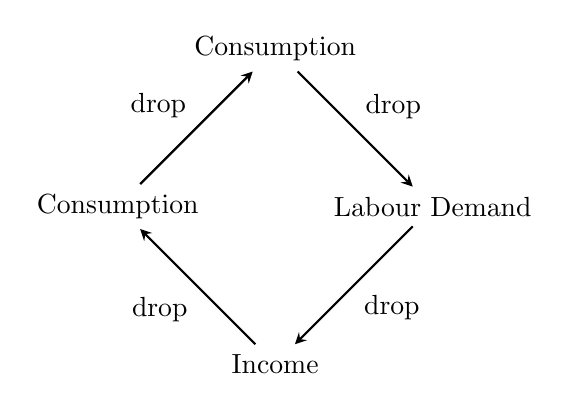
\begin{tikzpicture}[node distance=3cm, ->, >=stealth, thick]
            % Nodes placed in a circle
            \node (Consumption) at (0,2) {Consumption};
            \node (Labour Demand) at (2,0) {Labour Demand};
            \node (Income) at (0,-2) {Income};
            \node (back) at (-2,0) {Consumption};

            % Arrows with "drop" labels
            \draw[->] (Consumption) -- (Labour Demand) node[midway, above right] {drop};
            \draw[->] (Labour Demand) -- (Income) node[midway, below right] {drop};
            \draw[->] (Income) -- (back) node[midway, below left] {drop};
            \draw[->] (back) -- (Consumption) node[midway, above left] {drop};
        \end{tikzpicture}
        \caption*{Recession Cycle (Negative Feedback)}
    \end{minipage}
    \hfill
    \begin{minipage}{0.45\textwidth}
        \centering
        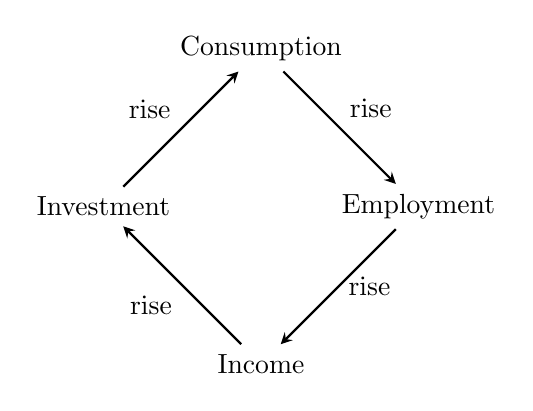
\begin{tikzpicture}[node distance=3cm, ->, >=stealth, thick]
            % Positive (recovery) cycle
            \node (consumption) at (0,2) {Consumption};
            \node (employment) at (2,0) {Employment};
            \node (investment) at (-2,0) {Investment};
            \node (income) at (0,-2) {Income};

            % Arrows with "rise" labels
            \draw[->] (consumption) -- (employment) node[midway, above right] {rise};
            \draw[->] (employment) -- (income) node[midway, right] {rise};
            \draw[->] (income) -- (investment) node[midway, below left] {rise};
            \draw[->] (investment) -- (consumption) node[midway, above left] {rise};
        \end{tikzpicture}
        \caption*{Recovery Cycle (Positive Feedback)}
    \end{minipage}
\end{figure}